\chapter{導入程式}
\section{bubbleRob與感測器於球場內程式}
\begin{figure}[hbt!]
\begin{center}
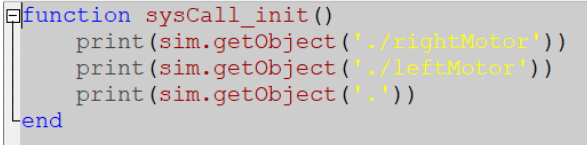
\includegraphics[width=16cm]{偵測}
\caption{\Large 偵測用於遠端操控的bubbleRob以及左右馬達的變值}\label{偵測用於遠端操控的bubbleRob以及左右馬達的變值}
\end{center}
\end{figure} 
\begin{figure}[hbt!]
\begin{center}
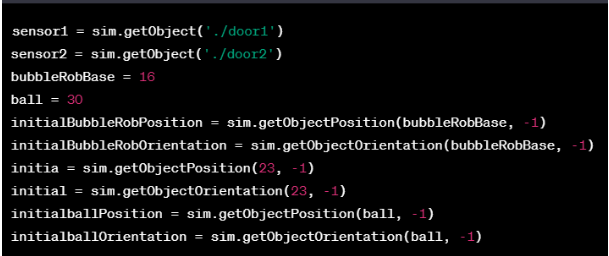
\includegraphics[width=16cm]{設定sensor}
\caption{\Large 設定sensor1、2為door1、2}\label{設定sensor1、2為door1、2}
\end{center}
\end{figure} 
\begin{figure}[hbt!]
\begin{center}
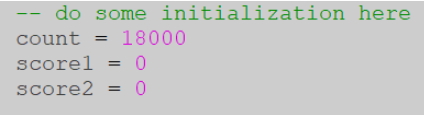
\includegraphics[width=16cm]{時間及得分}
\caption{\Large 計時器時間及得分設定}\label{計時器時間及得分設定}
\end{center}
\end{figure} 
\begin{figure}[hbt!]
\begin{center}
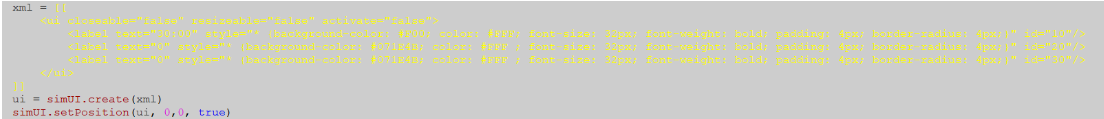
\includegraphics[width=16cm]{設定ui}
\caption{\Large 設定UI介面}\label{設定UI介面}
\end{center}
\end{figure} 
\newpage
\begin{figure}[hbt!]
\begin{center}
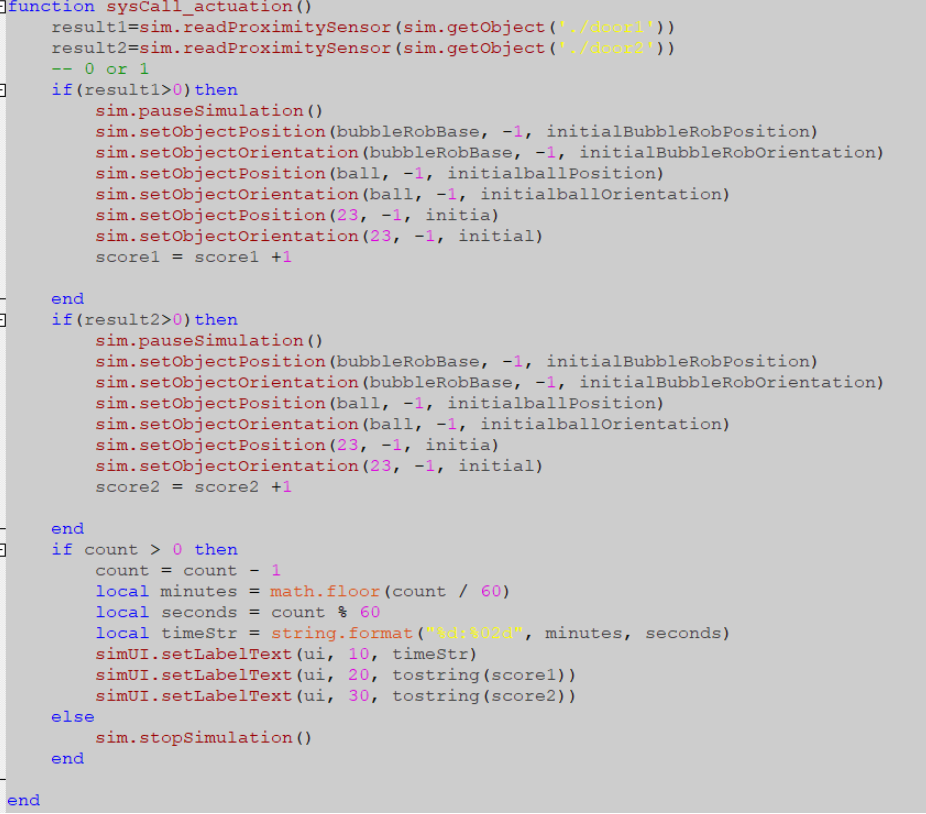
\includegraphics[width=16cm]{感測器偵測}
\caption{\Large 感測器偵測到物體UI介面加分及位置重製}\label{感測器偵測到物體UI介面加分及位置重製}
\end{center}
\end{figure} 
如(圖.\ref{偵測用於遠端操控的bubbleRob以及左右馬達的變值}):
第2行這個語句呼叫了sim.getObject函數並傳入了一個字串參數'./rightMotor'。這個函數是用於獲取場景中指定名稱的物體也就是我們的右馬達。print函數則是用於將獲取到的物體對象打印出來,以便進一步進行調試或是測試。
第3行這個語句和第一個語句類似,只是傳入的參數不同,這個函數是用於獲取場景中另一個名稱為leftMotor的物體也就是左馬達。
第4行這個語句呼叫了sim.getObject函數並傳入了一個字串參數'.'。這個參數代表獲取當前場景中的根對象。這個函數用於獲取當前場景的根對象,以便進行對場景的操作或是進一步獲取子對象。
函數 sysCallinit 用於初始化仿真環境和一些變量,而函數 sysCallactuation 用於執行機器人的運動和動作
,以及更新計時器和得分標籤的顯示。\\

如(圖.\ref{設定sensor1、2為door1、2}):
sensor1 和 sensor2 變量是用來存儲兩個傳感器的句柄,這些傳感器可能被機器人用來檢測周圍環境。
bubbleRobBase 變量存儲了機器人的基座句柄。
ball 變量存儲了一個球的句柄。
initialBubbleRobPosition 和 initialBubbleRobOrientation 分別是機器人基座的初始位置和方向。
initialballPosition 和 initialballOrientation 分別是球的初始位置和方向。\\

如(圖.\ref{計時器時間及得分設定}):
這段代碼用於進行一些初始化操作。具體來說,我們將一個名為 count 的變量初始化為 18000,
這個變量用於存儲倒計時的剩餘時間,單位為秒。我們還將 score1 和 score2 變量初始化為 0,
這兩個變量用於表示兩個玩家的得分。\\

如(圖.\ref{設定UI介面}):
這段程式碼是用來建立一個使用者介面 UI,讓使用者可以看到遊戲時間和兩方的得分。
程式中使用了XML格式的字串來定義介面的樣式,其中包括了三個標籤Label,分別是時間、玩家1得分和玩家2得分
並為每個標籤Label指定了一個唯一的識別碼 ID。
程式中的 ... 語法是 Lua 的多行字串表示法,可以方便地在一段文字中包含多行內容。
在這裡使用  ...  語法定義了一個名為 xml 的多行字串,這個字串中包含了UI元素的定義。
接下來,程式呼叫 simUI.create xml 方法來創建一個使用者介面,ui 變數存儲了返回值,這個返回值是介面的識別碼 ID 。
接著,程式呼叫simUI.setPosition ui, 0,0, true 方法來設定介面的位置,這裡將介面的位置設定為左上角,即 x 和 y 座標都為 0。\\

如(圖.\ref{感測器偵測到物體UI介面加分及位置重製}):
接下來是 sysCallactuation 函數,這個函數會在每一幀被調用。這個函數會檢測兩個門的狀態,如果某個門被打開了,那麼就暫停遊戲,並重置機器人和球的位置,以及增加對應玩家的得分。
另外,如果遊戲時間已經用完,那麼也會停止遊戲。在每一幀結束時,還會更新遊戲時間和得分在用戶界面上的顯示。
最後,需要注意的是,這些代碼並不是獨立運行的,而是作為一段代碼塊被嵌入到了一個名為 BubbleRob 的場景中。因此,在運行這段代碼之前,需要先打開這個場景。
\begin{figure}[hbt!]
\begin{center}
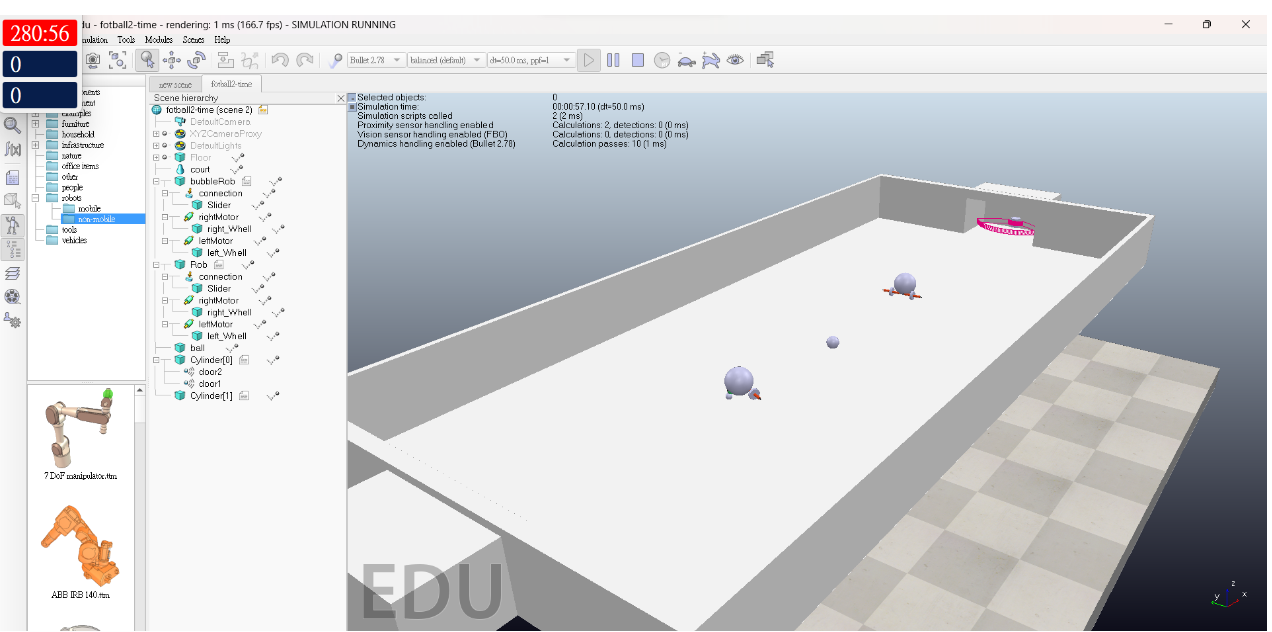
\includegraphics[width=16cm]{UI介面展示}
\caption{\Large 完成後UI介面展示}\label{完成後UI介面展示}
\end{center}
\end{figure} 
\section{本地程式}
\begin{figure}[hbt!]
\begin{center}
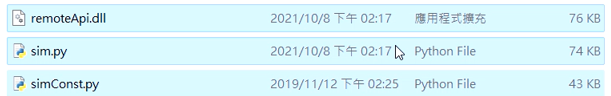
\includegraphics[width=16cm]{導入程式}
\caption{\Large 導入python程式}\label{導入python程式}
\end{center}
\end{figure} 
連機須將這三個檔案丟入python310內,如(圖.\ref{導入python程式})。
\begin{figure}[hbt!]
\begin{center}
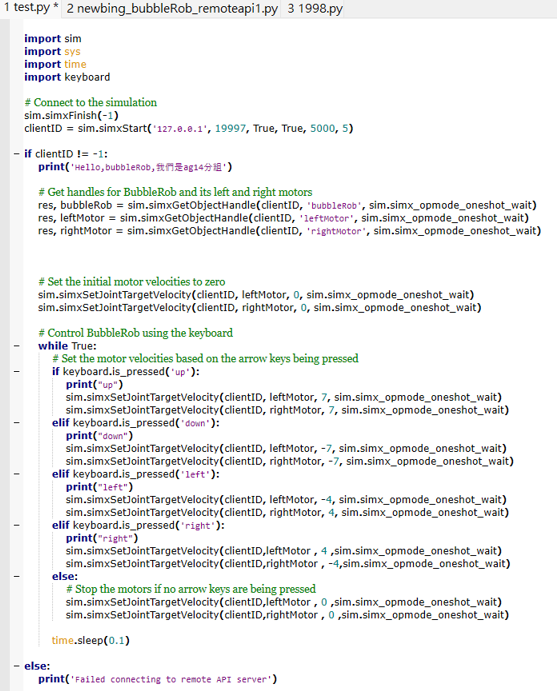
\includegraphics[width=16cm]{997}
\caption{\Large 本地控制程式}\label{本地控制程式}
\end{center}
\end{figure} 
\begin{figure}[hbt!]
\begin{center}
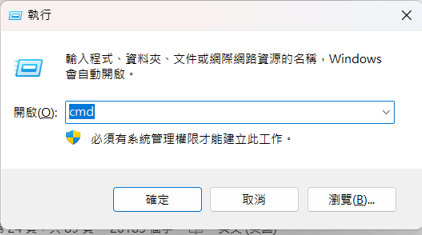
\includegraphics[width=16cm]{cmd}
\caption{\Large 查看本地IP}\label{查看本地IP}
\end{center}
\end{figure} 
\begin{figure}[hbt!]
\begin{center}
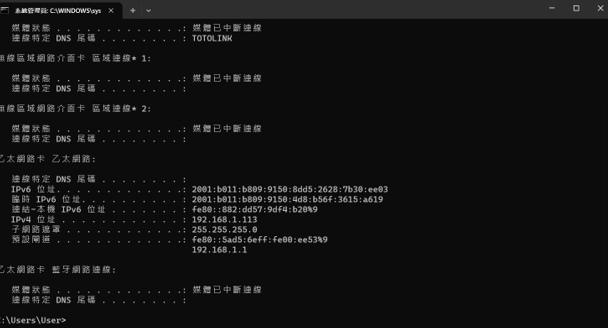
\includegraphics[width=16cm]{IP}
\caption{\Large IP config}\label{IP config}
\end{center}
\end{figure} 
\section{遠端程式}
\begin{figure}[hbt!]
\begin{center}
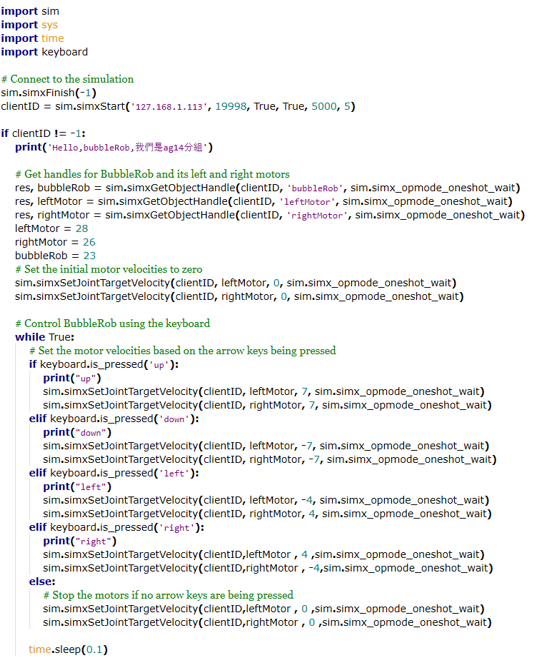
\includegraphics[width=16cm]{遠端程式}
\caption{\Large 遠端控制程式}\label{遠端控制程式}
\end{center}
\end{figure} 
如(圖.\ref{遠端控制程式}),須注意端口須改為19998。並且在leftMotor、rightMotor、bubbleRob輸入剛剛偵測的變值。